

\chapter{The Seifert-Van Kampen Theorem}

Theorem 15.5 Let \(K = {K}_{1} \cup  {K}_{2}\) be the union of two path-connected open sets, where \({K}_{1} \cap  {K}_{2}\) is also path-connected. Take \(b \in  {K}_{1} \cap  {K}_{2}\) , and suppose the group presentations for \({\pi }_{1}\left( {{K}_{1},b}\right) ,{\pi }_{1}\left( {{K}_{2},b}\right)\) are

\[
{\pi }_{1}\left( {{K}_{1},b}\right)  \cong  \left\langle  {{X}_{1} \mid  {R}_{1}}\right\rangle  ,\;{\pi }_{1}\left( {{K}_{2},b}\right)  \cong  \left\langle  {{X}_{2} \mid  {R}_{2}}\right\rangle  .
\]

Let the inclusions be

\[
{i}_{1} : {K}_{1} \cap  {K}_{2} \hookrightarrow  {K}_{1},\;{i}_{2} : {K}_{1} \cap  {K}_{2} \hookrightarrow  {K}_{2},
\]

then a presentation of \({\pi }_{1}\left( {K,b}\right)\) is given by:

\[
{\pi }_{1}\left( {K,b}\right)  \cong  \left\langle  {{X}_{1} \cup  {X}_{2} \mid  {R}_{1} \cup  {R}_{2} \cup  \left\{  {{\left( {i}_{1}\right) }_{ * }\left( g\right)  = {\left( {i}_{2}\right) }_{ * }\left( g\right)  : \forall g \in  {\pi }_{1}\left( {{K}_{1} \cap  {K}_{2},b}\right) }\right\}  }\right\rangle  .
\]

(Here \({\left( {i}_{1}\right) }_{ * } : {\pi }_{1}\left( {{K}_{1} \cap  {K}_{2},b}\right)  \hookrightarrow  {\pi }_{1}\left( {{K}_{1},b}\right)\) and \({\left( {i}_{2}\right) }_{ * } : {\pi }_{1}\left( {{K}_{1} \cap  {K}_{2},b}\right)  \hookrightarrow  {\pi }_{1}\left( {{K}_{2},b}\right)\) .)

\begin{itemize}
\item Example 15.4 1. Let \(K = {S}^{1} \land  {S}^{1}\) given by
\end{itemize}

\begin{center}
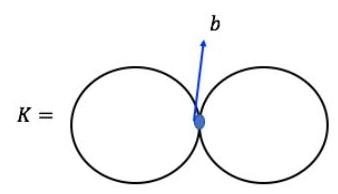
\includegraphics[max width=0.2\textwidth]{images/bo_d2bcsrref24c73avs720_149_787_508_338_194_0.jpg}
\end{center}
\hspace*{3em} 

(a) Then construct \(b\) as the intersection between two circles, and construct \({K}_{1},{K}_{2}\) as shown below: We can see that \({K}_{1} \cap  {K}_{2}\) is contractible:

\begin{center}
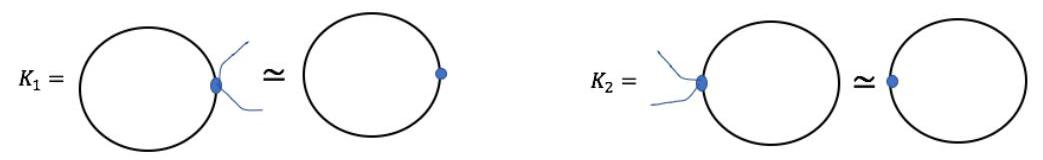
\includegraphics[max width=0.8\textwidth]{images/bo_d2bcsrref24c73avs720_149_448_1010_1043_160_0.jpg}
\end{center}
\hspace*{3em} 

\begin{center}
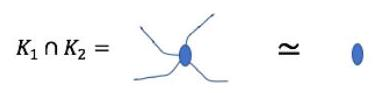
\includegraphics[max width=0.3\textwidth]{images/bo_d2bcsrref24c73avs720_149_780_1404_382_93_0.jpg}
\end{center}
\hspace*{3em} 

(b) As we have shown before, \({\pi }_{1}\left( {S}^{1}\right)  \cong  \mathbb{Z}\) , which follows that

\[
{\pi }_{1}\left( {{K}_{1},b}\right)  \cong  \langle \alpha \rangle ,\;{\pi }_{1}\left( {{K}_{2},b}\right)  \cong  \langle \beta \rangle
\]

\[
\text{ Also, }{\pi }_{1}\left( {{K}_{1} \cap  {K}_{2},b}\right)  \cong  {\pi }_{1}\left( {\{ b\} ,b}\right)  \cong  \{ e\} \text{ . }
\]

(c) It’s easy to compute \({\left( {i}_{1}\right) }_{ * }\) and \({\left( {i}_{2}\right) }_{ * }\) :

\({\left( {i}_{2}\right) }_{ * } : \;{\pi }_{1}\left( {{K}_{1} \cap  {K}_{2}}\right)  \rightarrow  {\pi }_{1}\left( {K}_{2}\right)\)

\[
\text{ with }e \mapsto  e
\]

with \(e \mapsto  e\)

(d) Therefore, by Seifert-Van Kampen Theorem,

\[
{\pi }_{1}\left( {K,b}\right)  \cong  \langle \alpha ,\beta  \mid  e = e\rangle  \cong  \langle \alpha ,\beta \rangle
\]

2. By induction,

\[
{\pi }_{1}\left( {{ \land  }^{n}{S}^{1},b}\right)  \cong  \left\langle  {{a}_{1},\ldots ,{a}_{n}}\right\rangle
\]

For instance, the figure illustration for \({ \land  }^{4}{S}^{1}\) and the basepoint \(b\) is given below:

\begin{center}
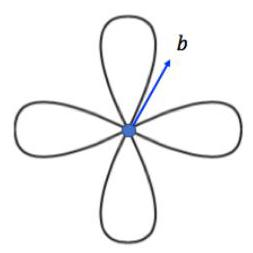
\includegraphics[max width=0.2\textwidth]{images/bo_d2bcsrref24c73avs720_150_700_767_253_253_0.jpg}
\end{center}
\hspace*{3em} 

3. (a) Construct \({S}^{2} = {K}_{1} \cup  {K}_{2}\) , which is shown below:

\begin{center}
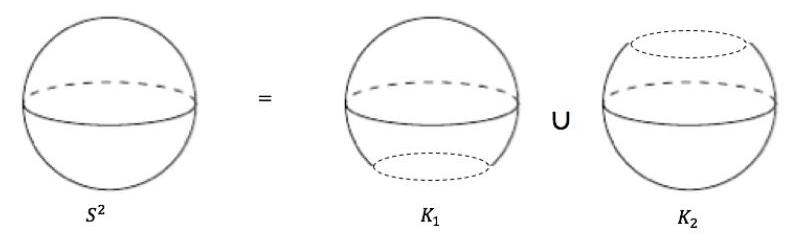
\includegraphics[max width=0.6\textwidth]{images/bo_d2bcsrref24c73avs720_150_424_1213_793_241_0.jpg}
\end{center}
\hspace*{3em} 

Therefore, we see that \({K}_{1} \cap  {K}_{2} \simeq  {S}^{1}\) :

\begin{center}
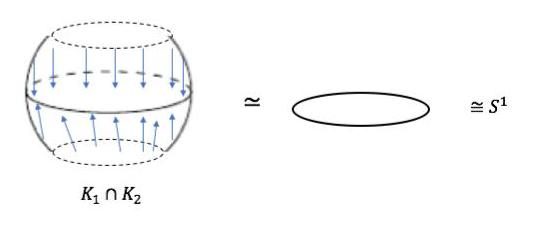
\includegraphics[max width=0.4\textwidth]{images/bo_d2bcsrref24c73avs720_150_562_1637_540_225_0.jpg}
\end{center}
\hspace*{3em} 

(b) It’s clear that \({K}_{1}\) and \({K}_{2}\) are contractible, and therefore

\[
{\pi }_{1}\left( {K}_{1}\right)  \cong  \langle \beta  \mid  \beta \rangle ,\;{\pi }_{1}\left( {K}_{2}\right)  \cong  \langle \gamma  \mid  \gamma \rangle
\]

and \({\pi }_{1}\left( {{K}_{1} \cap  {K}_{2}}\right)  \cong  {\pi }_{1}\left( {S}^{1}\right)  \cong  \langle \alpha \rangle\) .

(c) Then we compute \({\left( {i}_{1}\right) }_{ * }\) and \({\left( {i}_{2}\right) }_{ * }\) . In particular, the mapping \({\left( {i}_{1}\right) }_{ * }\) is defined as

\[
{\left( {i}_{1}\right) }_{ * } : \;{\pi }_{1}\left( {{K}_{1} \cap  {K}_{2}}\right)  \rightarrow  {\pi }_{1}\left( {K}_{1}\right)
\]

\[
\text{ with }\left\lbrack  \alpha \right\rbrack   \mapsto  \left\lbrack  {{i}_{1}\left( \alpha \right) }\right\rbrack
\]

where \(\alpha\) is any loop based at \(b\) . Since \({K}_{1}\) is contractible, we imply \(\alpha\) in \({K}_{1}\) is homotopic to \({c}_{b}\) , i.e.,

\[
{\left( {i}_{1}\right) }_{ * }\left( \left\lbrack  \alpha \right\rbrack  \right)  = \left\lbrack  {{i}_{1}\left( \alpha \right) }\right\rbrack   = e,\forall \alpha  \in  {\pi }_{1}\left( {{K}_{1} \cap  {K}_{2}}\right) .
\]

Similarly, \({\left( {i}_{2}\right) }_{ * }\left( \left\lbrack  \alpha \right\rbrack  \right)  = e\) .

(d) By Seifert-Van Kampen Theorem, we conclude that

\[
{\pi }_{1}\left( {S}^{2}\right)  \cong  \langle \beta ,\gamma  \mid  \beta ,\gamma ,e = e\rangle  \cong  \{ e\}
\]

4. Homework: Use the same trick to check that \({\pi }_{1}\left( {S}^{n}\right)  = \{ e\}\) for all \(n \geq  2\) . Hint: for \({S}^{3}\) , construct

\[
{K}_{1} = \left\{  {\left( {{x}_{1},\ldots ,{x}_{4}}\right)  \in  {S}^{3} \mid  {x}_{4} >  - 1/2}\right\}
\]

and

\[
{K}_{1} = \left\{  {\left( {{x}_{1},\ldots ,{x}_{4}}\right)  \in  {S}^{3} \mid  {x}_{4} < 1/2}\right\}
\]

5. (a) Consider the quotient space \(K \cong  {\mathbb{T}}^{2}\) , and we construct \(K = {K}_{1} \cup  {K}_{2}\) as follows:

\begin{center}
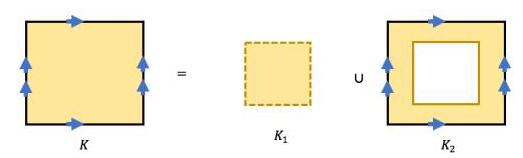
\includegraphics[max width=0.4\textwidth]{images/bo_d2bcsrref24c73avs720_151_718_1863_523_158_0.jpg}
\end{center}
\hspace*{3em} 

Therefore, we can see that \({K}_{1}\) is contractible, and \({K}_{2}\) is homotopy equivalent

to \({S}^{1} \land  {S}^{1}\) :

\begin{center}
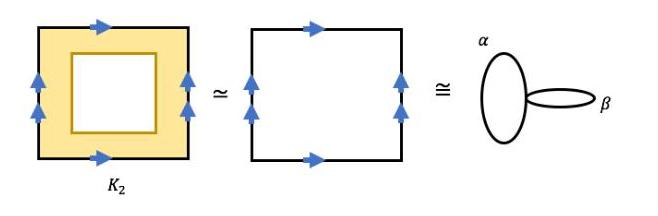
\includegraphics[max width=0.5\textwidth]{images/bo_d2bcsrref24c73avs720_152_507_433_658_216_0.jpg}
\end{center}
\hspace*{3em} 

Figure 15.2: Illustration for \({K}_{2} \simeq  {S}^{1} \land  {S}^{1}\)

and \({K}_{1} \cap  {K}_{2}\) is homotopic equivalent to the circle:

\begin{center}
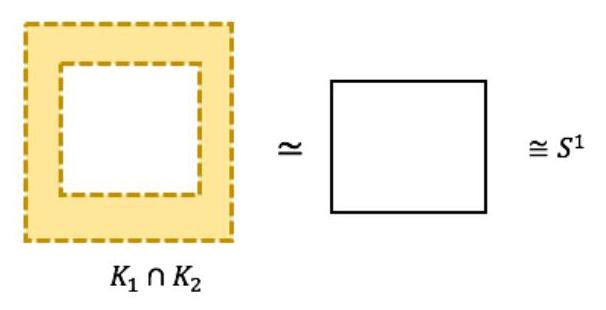
\includegraphics[max width=0.5\textwidth]{images/bo_d2bcsrref24c73avs720_152_532_877_606_310_0.jpg}
\end{center}
\hspace*{3em} 

(b) It follows that

\[
{\pi }_{1}\left( {K}_{1}\right)  \cong  \{ e\} ,\;{\pi }_{1}\left( {K}_{2}\right)  \cong  \langle \alpha ,\beta \rangle ,
\]

and \({\pi }_{1}\left( {{K}_{1} \cap  {K}_{2}}\right)  \cong  \langle \gamma \rangle\) .

(c) Then we compute \({\left( {i}_{1}\right) }_{ * }\) and \({\left( {i}_{2}\right) }_{ * }\) . In particular, \({\left( {i}_{1}\right) }_{ * }\) is trivial:

\[
{\left( {i}_{1}\right) }_{ * } : \;{\pi }_{1}\left( {{K}_{1} \cap  {K}_{2}}\right)  \rightarrow  {\pi }_{1}\left( {K}_{1}\right)
\]

\[
\text{ with }\left\lbrack  \alpha \right\rbrack   \mapsto  e
\]

Then compute \({\left( {i}_{2}\right) }_{ * }\) . In particular, for any loop \(\gamma\) , we draw the graph for \({i}_{2}\left( \gamma \right)\) :

\begin{center}
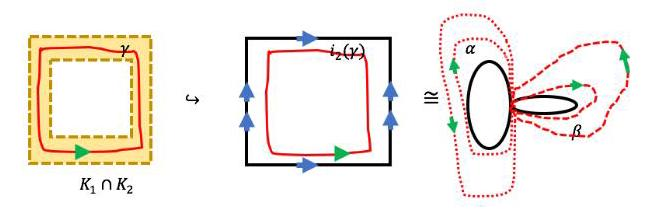
\includegraphics[max width=0.5\textwidth]{images/bo_d2bcsrref24c73avs720_153_650_353_651_212_0.jpg}
\end{center}
\hspace*{3em} 

Therefore,

\[
{\left( {i}_{2}\right) }_{ * }\left\lbrack  \gamma \right\rbrack   = \left\lbrack  {{i}_{2}\left( \gamma \right) }\right\rbrack   = \left\lbrack  {{\alpha \beta }{\alpha }^{-1}{\beta }^{-1}}\right\rbrack
\]

(d) By Seifert-Van Kampen Theorem, we conclude that

\[
{\pi }_{1}\left( K\right)  \cong  \left\langle  {\alpha ,\beta  \mid  \beta ,{\alpha \beta }{\alpha }^{-1}{\beta }^{-1} = e}\right\rangle   \cong  \langle \alpha ,\beta  \mid  ,{\alpha \beta } = {\beta \alpha }\rangle  \cong  \mathbb{Z} \times  \mathbb{Z}
\]

6. Exerise: The Klein bottle \(K\) shown in graph below satisfies \({\pi }_{1}\left( K\right)  = \left\langle  {a,b \mid  {ab}{a}^{-1}b}\right\rangle\) .

\begin{center}
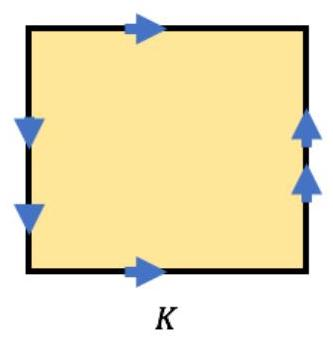
\includegraphics[max width=0.2\textwidth]{images/bo_d2bcsrref24c73avs720_153_825_1135_333_338_0.jpg}
\end{center}
\hspace*{3em} 

7. Consider the quotient space \(K = \mathbb{R}{P}^{2}\) . We construct \(K = {K}_{2} \cup  {K}_{2}\) , which is shown below:

\begin{center}
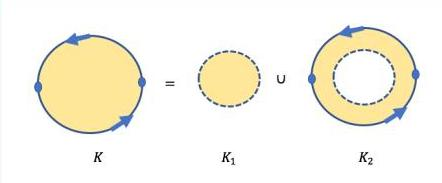
\includegraphics[max width=0.3\textwidth]{images/bo_d2bcsrref24c73avs720_153_757_1721_442_183_0.jpg}
\end{center}
\hspace*{3em} 

(a) It’s clear that \({K}_{1}\) is contractible. In hw3, question 1, we can see that \({K}_{2} \simeq  {S}^{1}\) . Moreover, similar as in (5), \({K}_{1} \cap  {K}_{2} \simeq  {S}^{1}\) .

(b) Therefore, \({\pi }_{1}\left( {K}_{1}\right)  = \{ e\}\) and \({\pi }_{1}\left( {K}_{2}\right)  = \langle \alpha \rangle ,{\pi }_{1}\left( {{K}_{1} \cap  {K}_{2}}\right)  = \langle \gamma \rangle\) .

(c) It’s easy to see that \({\left( {i}_{1}\right) }_{ * }\left( \left\lbrack  \gamma \right\rbrack  \right)  = e\) for any loop \(\gamma\) . For any loop \(\gamma\) , we draw the graph for \({i}_{2}\left( \gamma \right)\) :

\begin{center}
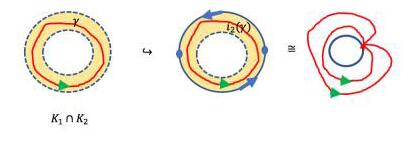
\includegraphics[max width=0.3\textwidth]{images/bo_d2bcsrref24c73avs720_154_638_533_407_144_0.jpg}
\end{center}
\hspace*{3em} 

Therefore, \({\left( {i}_{2}\right) }_{ * }\left( \left\lbrack  \gamma \right\rbrack  \right)  = \left\lbrack  {{i}_{2}\left( \gamma \right) }\right\rbrack   = \left\lbrack  {\alpha }^{2}\right\rbrack\) .

(d) By Seifert-Van Kampen Theorem, we conclude that

\[
{\pi }_{1}\left( K\right)  \cong  \left\langle  {\alpha  \mid  {\alpha }^{2} = e}\right\rangle   \cong  \mathbb{Z}/2\mathbb{Z} \cong  \{ 0,1{\} }_{\;\operatorname{mod}\;\left( 2\right) }
\]

8. Let \(K = {\mathbb{R}}^{2} \smallsetminus  \{ 2\) points \(\alpha ,\beta \}\) . As have shown in hw3, \(K \simeq  {S}^{1} \land  {S}^{1}\) , which implies

\[
{\pi }_{1}\left( K\right)  \cong  {\pi }_{1}\left( {{S}^{1} \land  {S}^{1}}\right)  \cong  \langle \alpha ,\beta \rangle .
\]

We can compute the fundamental group for \(K\) directly. Construct \(K = {K}_{1} \cup  {K}_{2}\) as follows:

\begin{center}
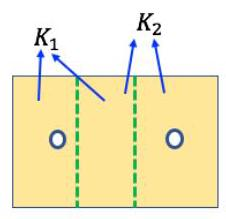
\includegraphics[max width=0.2\textwidth]{images/bo_d2bcsrref24c73avs720_154_702_1411_226_219_0.jpg}
\end{center}
\hspace*{3em} 

\(K\)

(a) It’s clear that \({K}_{1} \cong  {\mathbb{R}}^{2} \smallsetminus  \{\) one point \(\}  \simeq  {S}^{1}\) and similarly \({K}_{2} \simeq  {S}^{1}\) . Moreover, \({K}_{1} \cap  {K}_{2}\) is contractible

(b) Therefore,

\[
{\pi }_{1}\left( {K}_{1}\right)  \cong  \langle \alpha \rangle ,\;{\pi }_{1}\left( {K}_{2}\right)  \cong  \langle \beta \rangle ,\;{\pi }_{1}\left( {{K}_{1} \cap  {K}_{2}}\right)  \cong  \{ e\}
\]

(c) Therefore, \({\left( {i}_{1}\right) }_{ * }\) and \({\left( {i}_{2}\right) }_{ * }\) is trivial since \({\pi }_{1}\left( {{K}_{1} \cap  {K}_{2}}\right)  \cong  \{ e\}\) .

(d) By Seifert-Van Kampen Theorem, we conclude that

\[
{\pi }_{1}\left( K\right)  \cong  \langle \alpha ,\beta  \mid  e = e\rangle  \cong  \langle \alpha ,\beta \rangle
\]